%%% LaTeX Template: Two column article
%%%
%%% Source: http://www.howtotex.com/
%%% Feel free to distribute this template, but please keep to referal to http://www.howtotex.com/ here.
%%% Date: February 2011

%%% Preamble
\documentclass[	DIV=calc,%
							paper=a4,%
							fontsize=12pt,%
							onecolumn]{scrartcl}	 					% KOMA-article class

\usepackage{lipsum}													% Package to create dummy text
\usepackage[brazil]{babel}										% English language/hyphenation
\usepackage[protrusion=true,expansion=true]{microtype}				% Better typography
\usepackage{amsmath,amsfonts,amsthm}					% Math packages
\usepackage[pdftex]{graphicx}									% Enable pdflatex
\usepackage[svgnames]{xcolor}									% Enabling colors by their 'svgnames'
\usepackage[hang, small,labelfont=bf,up,textfont=it,up]{caption}	% Custom captions under/above floats
\usepackage{epstopdf}												% Converts .eps to .pdf
\usepackage{subfig}													% Subfigures
\usepackage{booktabs}												% Nicer tables
\usepackage{fix-cm}													% Custom fontsizes
\usepackage[utf8]{inputenc}
\usepackage[top=2.5cm, bottom=2.5cm, left=2.5cm, right=2.5cm]{geometry}
\usepackage[ddmmyyyy]{datetime}
\addto\captionsenglish{%
	\renewcommand\tablename{Tabela}
	\renewcommand\figurename{Figura}
} 
 

 
%%% Custom sectioning (sectsty package)
\usepackage{sectsty}													% Custom sectioning (see below)
\allsectionsfont{%															% Change font of al section commands
	\usefont{OT1}{phv}{b}{n}%										% bch-b-n: CharterBT-Bold font
	}

\sectionfont{%																% Change font of \section command
	\usefont{OT1}{phv}{b}{n}%										% bch-b-n: CharterBT-Bold font
	}



%%% Headers and footers
\usepackage{fancyhdr}												% Needed to define custom headers/footers
	\pagestyle{fancy}														% Enabling the custom headers/footers
\usepackage{lastpage}	

% Header (empty)
\lhead{}
\chead{}
\rhead{}
% Footer (you may change this to your own needs)

%% ====================================
%% ====================================
%% mude o rodape  do projeto
%% ====================================
%% ====================================

\lfoot{\footnotesize \texttt{Cabeamento estruturado}}


\cfoot{}
\rfoot{\footnotesize página \thepage\ de \pageref{LastPage}}	% "Page 1 of 2"
\renewcommand{\headrulewidth}{0.0pt}
\renewcommand{\footrulewidth}{0.4pt}



%%% Creating an initial of the very first character of the content
\usepackage{lettrine}
\newcommand{\initial}[1]{%
     \lettrine[lines=3,lhang=0.3,nindent=0em]{
     				\color{DarkGoldenrod}
     				{\textsf{#1}}}{}}



%%% Title, author and date metadata
\usepackage{titling}															% For custom titles

\newcommand{\HorRule}{\color{DarkGoldenrod}%			% Creating a horizontal rule
									  	\rule{\linewidth}{1pt}%
										}

\pretitle{\vspace{-30pt} \begin{flushleft} \HorRule 
				\fontsize{50}{50} \usefont{OT1}{phv}{b}{n} \color{DarkRed} \selectfont 
				}

\title{Projeto de cabeamento estruturado para biblioteca da UFOPR}					% Title of your article goes here

%% ====================================



\posttitle{\par\end{flushleft}\vskip 0.5em}

\preauthor{\begin{flushleft}
					\large \lineskip 0.5em \usefont{OT1}{phv}{b}{sl} \color{DarkRed}}
\author{Matheus Garcia Bessegato}  	% Author name goes here


\postauthor{\footnotesize \usefont{OT1}{phv}{m}{sl} \color{Black} 
					\\Universidade Tecnológica Federal do Paraná - Câmpus Cornélio Procópio 								% Institution of author
					\par\end{flushleft}\HorRule}

\date{}																				% No date




%%% Begin document
\begin{document}
\maketitle
\thispagestyle{fancy} 	
\thispagestyle{empty}		% Enabling the custom headers/footers for the first page 
% The first character should be within \initial{}




%% ====================================
%% ====================================
%% mude o resumo  do projeto
%% ====================================
%% ====================================
\initial{O}\textbf{ presente documento descreve o projeto de cabeamento estruturado de uma biblioteca para uma universidade fictícia, que será chamada de UFOPR (Universidade Fictícia do Oeste do Paraná). O corrente projeto parte de uma proposta de planta física para a biblioteca e busca apresentar a elaboração da planta lógica, com todos os equipamentos passivos e ativos da rede, levantamento de quantidades e custo, plano de certificação da rede e orçamento, com base nos usuários do local e nas atividades que serão desenvolvidas no ambiente.}

%% ====================================
\begin{figure}
	\centering
	
\includegraphics{utfpr}
\end{figure}

\vspace{3cm}
\centerline{\textit{\textbf{\today}}}

\clearpage
    \renewcommand*\listfigurename{Lista de figuras}
\listoffigures

\renewcommand*\listtablename{Lista de tabelas}
\listoftables

\clearpage
\renewcommand{\contentsname}{Sumário}
\tableofcontents
\clearpage

%% ====================================
%% ====================================
%% Inicio do texto
%% ====================================
%% ====================================
\section{Introdução}
A UFOPR é uma instituição fictícia localizada na região oeste do Paraná que conta com aproximadamente 800 alunos e 120 funcionários, entre professores e técnicos administrativos.

A instituição planeja construir uma biblioteca, adequada para incentivar e proporcionar conforto aos seus alunos e colaboradores. O novo ambiente contará com uma sala de estudos com 20 computadores e 8 computadores para funcionários, além de acesso sem fio à Internet e 6 ramais VoIP. O ambiente será monitorado por 8 câmeras IP internas.

O atual parque tecnológico da universidade conta com ao menos um computador para cada funcionário, um computador por sala de aula, 6 laboratórios com 41 computadores cada, cobertura Wi-Fi em todo o ambiente administrativo, salas de professores, laboratórios e em salas de aula, monitoramento com 60 câmeras IP e telefonia VoIP com 100 ramais. Os switches são todos gerenciáveis, 10/100 ou 10/100/1000, com divisões em VLANs. O Data Center conta com dois racks de 42U, dois switches CISCO 3750x, Distribuidor Interno Óptico (DIO), um link de dados de 100Mbps, um Storage NetApp com duas gavetas de expansão, com capacidade de armazenamento aproximada de 50TB e 4 servidores Dell virtualizados, destinados a prover os serviços de impressão, \textit{Active Directory}, \textit{gateway}, antivírus, VoIP, sistema de monitoramento de câmeras, ambiente de ensino a distância, dentre outros.

O presente documento abrange o projeto físico e lógico da biblioteca, as necessidades para a nova biblioteca, os benefícios de sua construção e implantação, um memorial descritivo dos equipamentos passivos que serão utilizados, planilha de orçamentos de materiais, cronograma de implantação, plano de certificação, plano de riscos e plano de manutenção.

\subsection{Benefícios}

A execução desse projeto trará maior conforto para os usuários e colaboradores da biblioteca da universidade, bem como deve melhorar a qualidade da aprendizagem, com a oferta de um grande número de computadores para estudo e a oferta de rede sem fio para a conexão com equipamentos pessoais. A concorrência por espaço e equipamentos será pequena ou inexistente e a qualidade do serviço oferecido será agradável aos usuários.

\section{Estado atual}

Atualmente, não existe um espaço adequado para estudos e pesquisas dentro da instituição, o que é uma das principais reclamações dos alunos, que ficam disputando horários nos computadores dos laboratórios para realizarem suas atividades. A falta de estrutura física e lógica para instalação de novos computadores e para os livros será solucionada com a execução do presente projeto na nova biblioteca.

\section{Requisitos}
A biblioteca deverá oferecer um ambiente propício ao estudo e à pesquisa, além de ferramentas atualizadas e acesso à Internet Gigabit para todos alunos e colaboradores.

\section{Usuários e Aplicativos}
 
\subsection{Usuários}
Os usuários da biblioteca podem ser classificados em dois tipos: estudantes ou colaboradores.

O número de estudantes da universidade, como informado anteriormente, está próximo a 800 e não há uma estimativa de aumento desse número devido ao espaço físico total da universidade não ser capaz de captar mais alunos e/ou turmas/cursos, logo, estima-se que o número de 20 computadores será capaz de suprir a demanda total da universidade.

Com a construção da nova biblioteca, estima-se que o número de colaboradores do setor poderá ser de até 08, o que já é calculado no presente projeto.

Como o número geral de usuários e equipamentos não deve ser alterado além do estimado, não haverá necessidade de aumento no número de pontos de rede e equipamentos. 

\subsection{Aplicativos}
Para o desenvolvimento das atividades de pesquisa e execução de aplicativos para demais trabalhos acadêmicos, os alunos necessitam de conexão Ethernet Gigabit.

Para acesso aos sistemas da universidade e da biblioteca, os colaboradores necessitam também de conexão Ethernet Gigabit.

\section{Estrutura predial}
A planta física da biblioteca contempla todos os requisitos dos usuários e aplicativos. A figura 1 mostra a planta do local com a localização de todas as salas e móveis que devem ser utilizados no local.

\begin{figure}[h!]
	\centering
	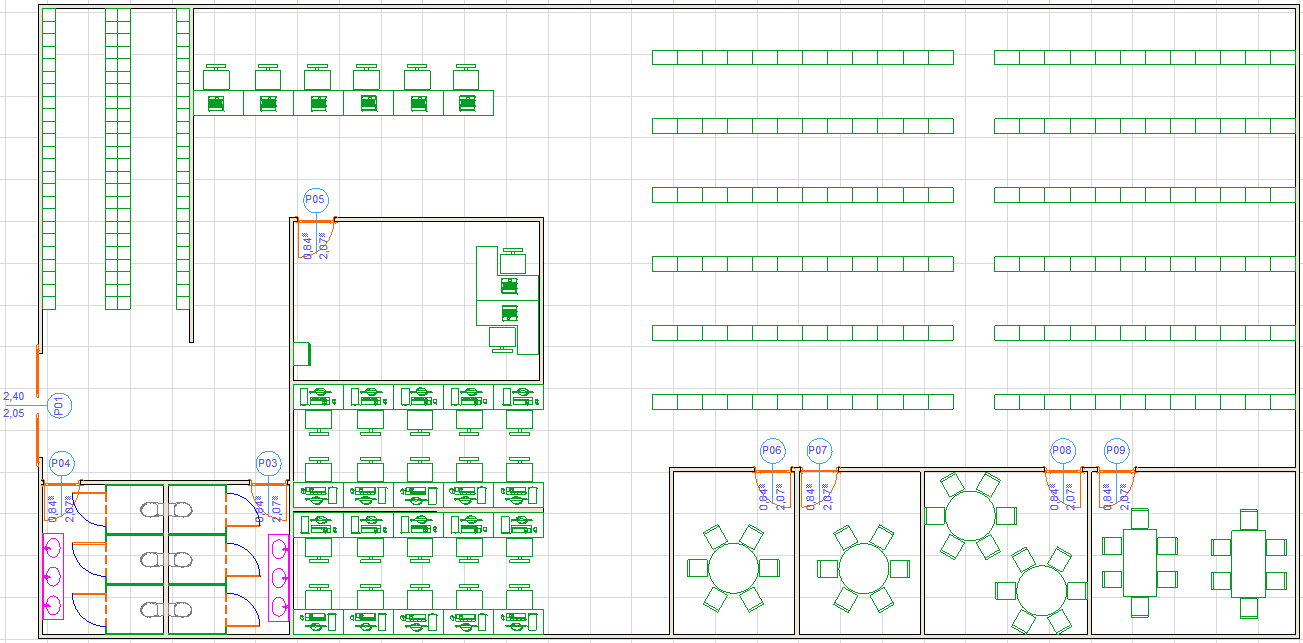
\includegraphics[width=\textwidth]{planta-fisica}
	\caption{Planta física da biblioteca da UFOPR.}
	\label{planta-fisica}
\end{figure}

O prédio possui 450 metros quadrados (15m x 30m), dividido entre dois banheiros, armários guarda-volumes, balcão de atendimento aos usuários, sala de processamento técnico (sala mais ao centro do prédio), área de estudos com computadores, quatro salas de estudos em grupo e área de prateleiras de livros.

O rack ficará na sala de processamento técnico da biblioteca, ambiente com maior restrição de acesso e mais centralizado. A direita do rack ficará a área de estudos com 20 computadores e a esquerda a área de atendimento aos usuários, com 8 computadores. Dentro da sala de processamento técnico haverão 2 computadores. Os pontos de rede mais distantes e isolados serão os pontos das câmeras e \textit{Access Points}, sendo o mais distante a aproximadamente 35m . Nas salas de estudo em grupo não haverá ponto de rede cabeada, apenas sinal de Internet sem fio.

\section{Planta Lógica - Elementos estruturados}

\subsection{Topologia}

O diagrama básico da interligação da rede da UFOPR é mostrado na figura 2.

\begin{figure}[h!]
	\centering
	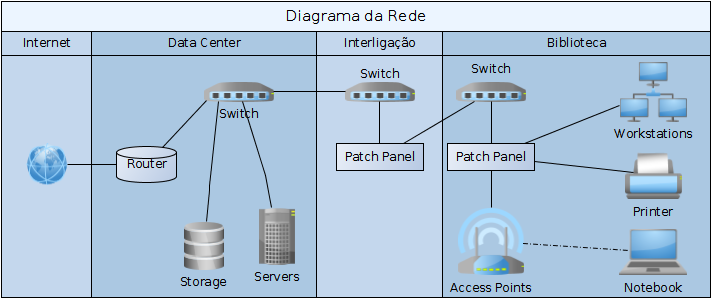
\includegraphics[width=\textwidth]{diagramaRede}
	\caption{Diagrama de interligação da rede da UFOPR.}
	\label{diagramaRede}
\end{figure}

É possível observar na figura 2, basicamente, como são realizadas as interligações da rede. O link de fibra óptica chega pela \textit{Entrance Facility} até a \textit{Equipament Room} (Data Center), onde, por meio do \textit{Backbone Cabling} conecta a \textit{Equipament Room} à \textit{Telecommunication Room} (Interligação). Há também um segundo \textit{Backbone Cabling} até a \textit{Telecommunication Room} da bilioteca, local em que parte o \textit{Horizontal Cabling} até as \textit{Work Areas}, para conectar os dispositivos finais.

Por não se tratar de um setor crítico para o funcionamento da universidade, os investimentos não serão tão acentuados, não havendo, por exemplo, redundância no link que conecta-se à biblioteca. Caso haja um rompimento de fibra, não haverá conexão até a solução do problema.

Os pontos de rede seguirão das áreas de trabalho e serão conectorizados em um Patch Panel no rack que estará instalado na sala de processamento técnico da biblioteca. 

A figura 3 mostra a planta da rede lógica da biblioteca da UFOPR.
\begin{figure}[h!]
	\centering
	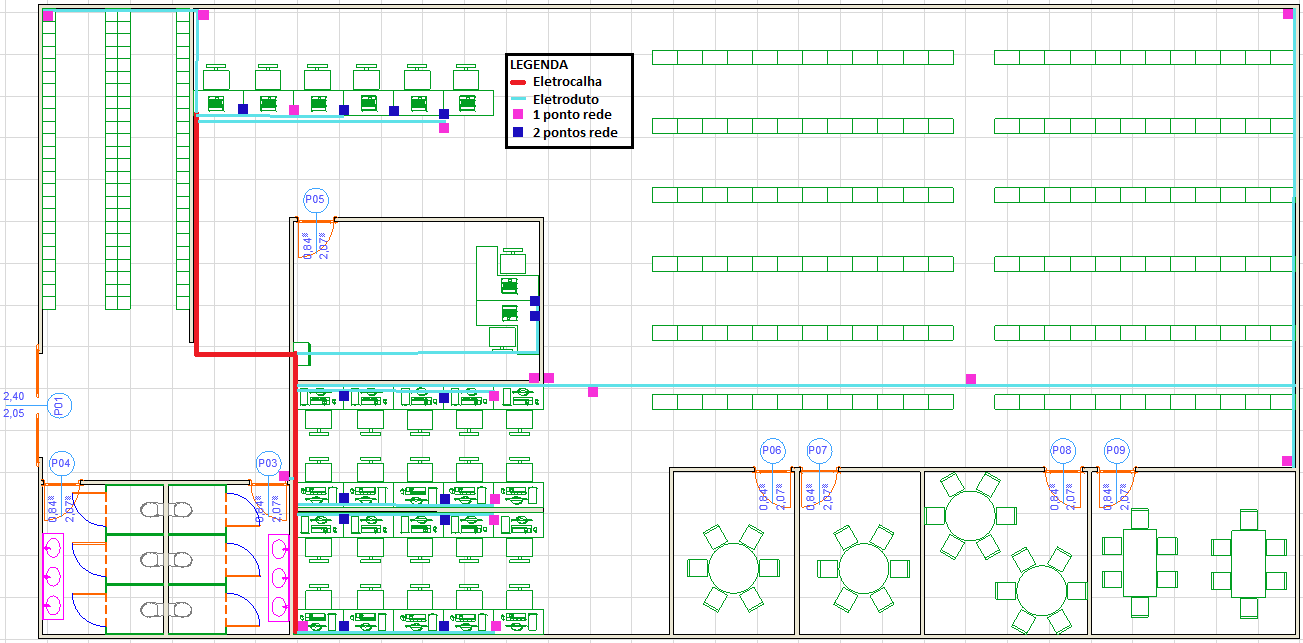
\includegraphics[width=\textwidth]{planta-logica}
	\caption{Planta da rede lógica da biblioteca da UFOPR.}
	\label{planta-logica}
\end{figure}

Nota-se que as eletrocalhas partem do rack, mais centralizado na edificação, e distribui-se por meio dos eletrodutos em seus 44 pontos de rede, contemplando toda a estrutura necessária para comunicação dos computadores, \textit{Access Points}, câmeras IP, e telefones VoIP.

\subsection{Encaminhamento}
Os cabos UTP de 4 pares categoria 6 serão encaminhados por meio de eletrocalhas instaladas acima do forro da biblioteca e então derivados em eletrodutos, tudo em alumínio, devidamente aterrados, que os conduzirão até as estações de trabalho.

\subsection{Memorial descritivo}

Os equipamentos passivos que serão utilizados, seguidos de seu tipo (quando houver), fabricante (quando houver), e quantidade, respectivamente, estão relacionados abaixo:

\begin{itemize}
	\item Cabo UTP; categoria 6; Furukawa; 552m;
	\item \textit{Patch panel}; 48 portas categoria 6; Furukawa; 1 unidade;
	\item \textit{Patch cord}; 1,5m categoria 6; Furukawa; 88 unidades;
	\item DIO; multimodo; Furukawa; 1 unidade;
	\item Rack; 8U 19" de parede; Attic; 1 unidade;
	\item Organizador de cabos; 1U alta densidade; qualquer; 2 unidades;
\end{itemize}

\subsection{Identificação dos cabos}
Os cabos serão identificados seguindo o padrão de identificação de pontas de cabo da NBR14565 \cite{nbr}. O primeiro cabo será identificado como CY 01 01, sequencialmente, até o último como CY 01 44. 	

\section{Implantação}
A expectativa de duração da implantação está descrita na tabela 1:
\begin{table}[h!]
	\centering
	\caption{Cronograma de Implantação}
	\label{cronograma-implantacao}
	\begin{tabular}{ll}
		\multicolumn{2}{l}{\textbf{CRONOGRAMA DE IMPLANTAÇÃO}} \\
		\textbf{TAREFA}                & \textbf{DURAÇÃO}      \\
		Instalação dos condutores      & 12h                   \\
		Instalação dos cabos           & 8h                    \\
		Identificação dos cabos        & 3h                    \\
		Montagem do rack               & 5h                    \\
		Certificação                   & 2h                   
	\end{tabular}
\end{table}

\section{Plano de certificação}
Para certificação da rede, deverá primeiramente ser realizada uma análise visual do trabalho de instalação e então, com equipamento apropriado, deverão ser testados todos os segmentos de cabos, adotando os seguintes parâmetros:

\begin{itemize}
	\item Wire Map;
	\item Comprimento;
	\item Atenuação;
	\item Resistência e Capacitância;
	\item Next;
	\item PSNext;
	\item Return Loss;
	\item Fext;
	\item Elfext;
	\item PSELfext;
	\item Propagation Delay;
	\item Delay Skew.
\end{itemize}

A certificação de todos os segmentos deverá ser em conformidade com as normas para a categoria 6 e executada por uma empresa diferente da executante do projeto, buscando aumentar a confiabilidade dos testes executados no cabeamento. A certificação deverá ser executada, preferencialmente, na modalidade “Link permanente” e com a rede em uso.

Deverá ser entregue, ao final da certificação, um relatório para cada ponto e/ou segmento testado, informando o resultado do teste para cada parâmetro indicado.

\section{Plano de manutenção}
Por não se tratar de um local crítico, como citado anteriormente neste projeto, não haverá plano de manutenção, seja preventivo ou seja corretivo. As ações serão tomadas mediante entendimento da equipe de TI do local, conforme disponibilidade e necessidade.

\subsection{Plano de expansão}
O projeto contempla o que se espera como uso máximo da biblioteca e, por esse motivo, não se espera que haja expansão. Caso haja essa necessidade no futuro, o ativo de rede deverá ser suficiente para até mais três pontos de rede, necessitando troca ou acréscimo de equipamentos no caso de maior necessidade, perante estudos.

\section{Risco}
O projeto foi realizado com base nas demandas passadas pela insituição. Quaisquer alterações de \textit{layout} dos ambientes ou informação incorreta, poderá trazer problemas, especialmente no que tange a quantidade de pontos e a localização dos mesmos.

\section{Orçamento}
\begin{table}[h!]
	\centering
	\caption{Orçamentos}
	\label{orcamentos}
	\begin{tabular}{lccc}
		\multicolumn{4}{c}{\textbf{ORÇAMENTO}}                                                                                                                                             \\
		\textbf{ITEM}                     & \multicolumn{1}{l}{\textbf{VALOR}} & \multicolumn{1}{l}{\textbf{QUANTIDADE}} & \multicolumn{1}{l}{\textbf{TOTAL}}                              \\
		Cabo UTP Furukawa Cat. 6          & 710,00                             & 2 caixas                                & 1.420,00                                                        \\
		Patch Cord Furukawa Cat. 6 1,5m   & 19,00                              & 88                                      & 1.672,00                                                        \\
		DIO B48 Furukawa                  & 219,00                             & 1                                       & 219,00                                                          \\
		Cordão Óptico Multimodo Furukawa  & 29,00                              & 1                                       & 29,00                                                           \\
		Acoplador DIO                     & 12,00                              & 1                                       & 12,00                                                           \\
		Patch Panel 48p Furukawa Cat. 6   & 650,00                             & 1                                       & 650,00                                                          \\
		Rack 8U 19" Attic de parede       & 246,00                             & 1                                       & 246,00                                                          \\
		Organizador Cabos alta densidade. & 19,00                              & 2                                       & 38,00                                                           \\
		Switch Cisco 2960                 & 13.194,84                          & 1                                       & 13.194,84                                                       \\
		Access Point Cisco 3602           & 846,00                             & 2                                       & 1.692,00                                                        \\
		Câmera IP dome Axis               & 1399,20                            & 8                                       & 11.193,60                                                       \\
		Telefone IP Intelbrás TIP 125     & 193,00                             & 6                                       & 1.158,00                                                        \\
		RJ-45 Fêmea Furukawa Cat. 6       & 24,00                              & 44                                      & 1.056,00                                                        \\
		Certificação "Link Permanente"    & 74,75                              & 44                                      & 3.289,00                                                        \\
		Eletrocalha                       & 23,00                              & 15m                                     & 345,00                                                          \\
		Tampa                             & 16,00                              & 15m                                     & 240,00                                                          \\
		Eletroduto                        & 6,75                               & 78m                                     & 526,50                                                          \\
		Porta Equipamento + espelho       & 6,25                               & 30                                      & 187,50                                                          \\ \cline{4-4} 
		& \multicolumn{1}{l}{}               & \multicolumn{1}{l}{}                    & \multicolumn{1}{l}{37.168,44} 
	\end{tabular}
\end{table}

\section{Recomendações}
Recomenda-se que não sejam realizadas alterações no posicionamento dos pontos de rede sem antes consultar o projetista da rede, sob o risco de comprometer o cabeamento e, consequentemente, a certificação dos cabos e/ou segmentos alterados.
Recomenda-se não trocar ativos e passivos por outros de qualidade inferior, sob o risco de comprometer o funcionamento e/ou desempenho da rede.
No caso de quaisquer dúvidas sobre o projeto ou necessidades de ampliação, alteração ou reestruturação, consultar primeiramente o projetista.

\section{Referências bibliográficas}

\renewcommand\refname{} %%Referências bibliográficas}  
\bibliographystyle{ieeetr}
\bibliography{referencias}  

\end{document}